% 33-34(33쪽) — 34번 그림 · y=f(x) 의 그래프(증가하는 곡선 · x=2 에서 빈 점 · x=2, x=4 안내 점선). 스캔 화질이 낮아 TikZ 로 다시 그림.
% 원문에 있는 것만: x축 눈금 2, 4 · 빈 점 (2, f(2)) · 점선 두 줄 · 라벨 y=f(x), O, x, y (y축 눈금은 원문에 없다).
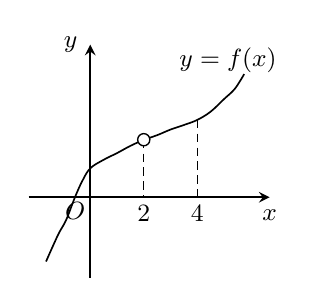
\begin{tikzpicture}[x=0.34cm, y=0.34cm, line width=0.6pt]
  \draw[->, >=stealth, line width=0.7pt] (-2.3,0) -- (6.7,0) node[below=1pt, font=\small] {$x$};
  \draw[->, >=stealth, line width=0.7pt] (0,-3.0) -- (0,5.7) node[left=1pt, font=\small] {$y$};
  \draw[densely dashed, line width=0.4pt] (2,2.15) -- (2,0);
  \draw[densely dashed, line width=0.4pt] (4,2.89) -- (4,0);
  \draw[line width=0.6pt] plot[smooth, tension=0.6] coordinates {(-1.65,-2.4) (-1.2,-1.4) (-0.9,-0.85) (-0.57,0) (-0.3,0.6) (0,1.08) (0.5,1.4) (1,1.65) (1.5,1.92) (2,2.15)};
  \draw[line width=0.6pt] plot[smooth, tension=0.6] coordinates {(2,2.15) (2.5,2.32) (3,2.53) (3.5,2.7) (4,2.89) (4.5,3.2) (5,3.67) (5.4,4.05) (5.75,4.6)};
  \draw[fill=white, line width=0.5pt] (2,2.15) circle (2.2pt);
  \node[font=\small, inner sep=2.5pt, below] at (2,0) {$2$};
  \node[font=\small, inner sep=2.5pt, below] at (4,0) {$4$};
  \node[font=\small, inner sep=1.5pt, below left] at (0,0) {$\pt{O}$};
  \node[font=\small, anchor=west, inner sep=1pt] at (3.2,5.1) {$y=f(x)$};
\end{tikzpicture}
